\documentclass [a4paper, 12pt] {article}

% ------------------------------------------------------------
% DO NOT CHANGE: BEGIN
% ------------------------------------------------------------

\usepackage[utf8]{inputenc}  
\usepackage[T1]{fontenc}  
\usepackage{lmodern}
\usepackage[english]{babel}
\usepackage{fancybox}
\usepackage{listings}
\usepackage{color}
\usepackage{graphicx,subfigure}
\usepackage[titletoc]{appendix}
\usepackage{float} % figures flottantes 
\usepackage{here} % figures flottantes
\usepackage{url}
\usepackage{enumitem}
\setlist[itemize]{noitemsep, nolistsep}
\setlist[enumerate]{noitemsep, nolistsep}
\usepackage{xcolor}
\usepackage[colorlinks=true]{hyperref}
\usepackage{tabularx}
\usepackage{minted}
\usepackage{amsmath}
\usepackage[skins,breakable]{tcolorbox}

% --------------------------------------------------------------
% Title
% --------------------------------------------------------------
\makeatletter
\newcommand\maintitle[1]{
    \quitvmode
    \hb@xt@\linewidth{
        \dimen@=1ex
        \advance\dimen@-2pt
        \leaders\hrule \@height1ex \@depth-\dimen@\hfill
        \enskip
        \textbf{#1}
        \enskip
        \leaders\hrule \@height1ex \@depth-\dimen@\hfill
    }
}
\makeatother

% --------------------------------------------------------------
% Some parameters
% --------------------------------------------------------------
\oddsidemargin =0 mm
\topmargin = -10 mm
\footskip = 20mm
\textheight = 240 mm 
\textwidth = 160mm

% --------------------------------------------------------------
% Q&A environments
% --------------------------------------------------------------

\newcommand{\emptyquestion}{Please fill this space with your question.}

\newcommand{\emptyanswer}{Please fill this space with your answer.}

\newcounter{question}

\definecolor{question_color}{RGB}{181,124,64}
\definecolor{question_color_fill}{RGB}{252,248,227}

\newcommand{\thequestionref}{No reference}

\makeatletter
\newenvironment{question}[1]
{
\refstepcounter{question}
\def\@currentlabel{{#1}}
\label{ref-question-\thequestion}
\addcontentsline{toc}{subsection}{{#1}}
\noindent
\begin{tcolorbox}[
    colframe=question_color,
    colback=question_color_fill,
    coltitle=question_color_fill,  
    title=\centering\textbf{Question #1:},
    breakable,
    width=\textwidth]
}
{   \end{tcolorbox}
}
\makeatother

\newenvironment{answer}
{
\noindent
{
\hypersetup{allcolors=question_color}
\flushleft
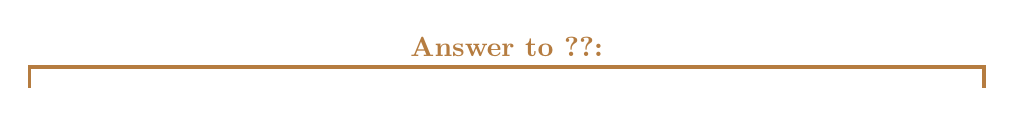
\begin{tikzpicture}
    \draw[very thick,question_color] (0,0) -- ++(0,+7.5pt)
    -- ++(\textwidth,0) node[midway,above] {\textbf{Answer to \ref{ref-question-\thequestion}:}}
    -- ++(0,-7.5pt);
\end{tikzpicture}
\vspace{-.3cm}
}
\begin{tcolorbox}[
    blanker,
    width=\textwidth,
    breakable]
}
{   \end{tcolorbox}
\vspace{-.4cm}
\flushleft

\begin{tikzpicture}
    \draw[very thick,question_color] (0,0) -- ++(0,-7.5pt)
    -- ++(\textwidth,0)
    -- ++(0,+7.5pt);
\end{tikzpicture}
}

\usepackage{tikz}

% --------------------------------------------------------------
% Code environments
% --------------------------------------------------------------
\usemintedstyle{borland}
\providecommand*{\listingautorefname}{Listing}

\newenvironment{python}
{\VerbatimEnvironment
\begin{minted}[
linenos,
% fontfamily=courier,
fontsize=\normalsize,
xleftmargin=21pt,
]{python}}
{\end{minted}}

\newcommand\py[1]{\mintinline{python}{#1}}

\newcommand\la[1]{\mintinline{latex}{#1}}

% --------------------------------------------------------------
% CELL environments
% --------------------------------------------------------------

\newcounter{cell}

\definecolor{cell_color}{RGB}{7,128,164}
\definecolor{cell_color_fill}{RGB}{247,247,247}

\newcommand{\thecellref}{No reference}

\makeatletter
\newenvironment{cell}[1]
{
\refstepcounter{cell}
\def\@currentlabel{{#1}}
\label{ref-cell-\thecell}
\addcontentsline{toc}{subsection}{\texttt{CELL N$^{\circ}${#1}}}
\noindent
\begin{tcolorbox}[
    colframe=cell_color,
    colback=cell_color_fill,
    coltitle=cell_color_fill,  
    title=\centering\texttt{CELL N$^{\circ}${#1}:},
    breakable,
    width=\textwidth]
}
{   \end{tcolorbox}
}
\makeatother

% ------------------------------------------------------------
% DO NOT CHANGE: END
% ------------------------------------------------------------
\begin{document}

    \begin{center}
        \Large
        \centering
        \maintitle{LEPL1109 - Statistics and Data Sciences}
        \textsc{\textbf{HACKATHON 3 - Bias in Clustering Algorithms}}\\
        \vspace{0.1cm}
         Group n°XX\hfill December 22, 2024 \\
       \noindent\hrulefill
    \end{center}
    \vspace*{0.5cm}

    % ------------------------------------------------------------
    % FILL WITH YOUR NAMES: BEGIN
    % ------------------------------------------------------------
    \hspace*{-0.75cm}
    \fbox{\parbox{\textwidth}{
    \begin{tabularx}{\textwidth}{X|X|c}
       \textbf{Lastname}  & \textbf{Firstname} & \textbf{Noma} \\
       \hline
        <Lastname 1> & <Firstname 1> & 11111111 \\
        <Lastname 2> & <Firstname 2> & 22222222 \\
        <Lastname 3> & <Firstname 3> & 33333333 \\
        <Lastname 4> & <Firstname 4> & 44444444 \\ 
        <Lastname 5> & <Firstname 5> & 55555555 \\ 
        <Lastname 6> & <Firstname 6> & 66666666 \\ 
    \end{tabularx}
    }}
    % ------------------------------------------------------------
    % FILL WITH YOUR NAMES: END
    % ------------------------------------------------------------

    \vspace*{0.5cm}
    
    \hrule
    
    \vspace*{0.5cm}
    
    Please carefully read the following guidelines:
    
    \begin{itemize}
        \item Answer in English, with complete sentences and correct grammar. Feel free to use grammar checker tools such as \href{https://languagetool.org/fr}{LanguageTools}.
        \item Do not modify questions, and input all answers inside \la{\begin{answer}...\end{answer}} environments.
        \item Each question should be followed by an answer.
        \item You are allowed (and often encouraged) to add figures that support your answers, provided that you explain how they support your claims.
        \item Clearly cite every source of information (even for pictures!).
        \item Whenever possible, use the \texttt{.pdf} format when you export your images (this usually makes your report look prettier).
    \end{itemize}

    {
    \hypersetup{allcolors=black}
    }   
    \clearpage

\renewcommand{\arraystretch}{0.84}

\begin{question}{1.1: Removing unnecessary features}
    Can you already, a priori, detect that some features are useless? If yes, list those (useless) features and explain your choice. If not, then explain why it is better to wait.

    Generally speaking, is it a good idea to remove a feature based on \emph{a priori} knowledge, or doesn't it alter the final outcome?
\end{question}
\begin{answer}\color{blue} 
% ------------------------------------------------------------
% TO FILL 
% ------------------------------------------------------------
\end{answer}

\begin{question}{1.2: Handling missing data}
    Given the dataset and the amount / type of missing information, what strategy do you propose to follow regarding missing data (NaNs) ? Justify briefly your choice.
\end{question}
\begin{answer}\color{blue} 
% ------------------------------------------------------------
% TO FILL 
% ------------------------------------------------------------
\end{answer}

\begin{question}{1.3: New features}
    What features have you added? If a particular manipulation has been applied, please explain.
\end{question}
\begin{answer}\color{blue} 
% ------------------------------------------------------------
% TO FILL 
% ------------------------------------------------------------
\end{answer}

\begin{question}{2.1: (Im)Balanced dataset ?}
Is the dataset imbalanced ? What could be the consequences in terms of fairness i.e. in terms of the model performing equally well across all groups ?
\end{question}
\begin{answer}\color{blue} 
% ------------------------------------------------------------
% TO FILL 
% ------------------------------------------------------------
\end{answer}

\begin{question}{2.2: Principal Component Analysis}
Do all features have the same importance? If no, which features are less important, and why ? You can use all other graphs from the visualization part to justify your answer.
\end{question}
\begin{answer}\color{blue}
% ------------------------------------------------------------
% TO FILL 
% ------------------------------------------------------------
\end{answer}

\begin{question}{3.1: Number of clusters}
Accounting for all features, what do you think is the ideal number of clusters ? What will happen if too many or too few clusters are chosen
\end{question}
\begin{answer} \color{blue}
% ------------------------------------------------------------
% TO FILL 
% ------------------------------------------------------------
\end{answer}

\begin{question}{3.2: Quality of the clustering}
You considered three different measures for the quality of the clustering: the first one is the silhouette score and is oblivious to the true labels: it is a truly unsupervised metric. The second and third metric use the true label to assess the quality of the clustering. Based on this observation,
\begin{enumerate}
    \item Comment on the evolution of each metric according to the number of clusters.
    \item Comment on what do you now think is the ideal number of clusters.
\end{enumerate}
\end{question}
\begin{answer}\color{blue}
% ------------------------------------------------------------
% TO FILL 
% ------------------------------------------------------------
\end{answer}

\begin{question}{4.1: Fairness of your model}
You considered two different measures for the fairness of your model and checked for various variants of your algorithm (number of clusters) the value of these fairness metrics.

Is your algorithm unfair ? If yes, which ethnic group is penalized by the unfairness of your model ?
\end{question}
\begin{answer}\color{blue}
% ------------------------------------------------------------
% TO FILL 
% ------------------------------------------------------------
\end{answer}

\begin{question}{4.2: Presence of the sensitive features in the dataset [BONUS]}
In Cell 1.5, you removed the sensitive features from your dataset before building your algorithm. Yet, you may have noticed unfairness in your algorithm.
\begin{enumerate}
    \item Provide reasons why it is not necessarily enough to remove sensitive features from your dataset if you want to have fair predictions.
    \item Compute FPR and Demographic Parity for your algorithm when trained on the full dataset. Is the fairness of your classifier worse ?
\end{enumerate}
\end{question}
\begin{answer}\color{blue}
% ------------------------------------------------------------
% TO FILL 
% ------------------------------------------------------------
\end{answer}

\begin{question}{5.1: Visualization}
Produce a clear, clean figure expressing a result or giving an overall vision of your work for this hackathon. Please feel free to do as you wish. Be original! The clarity, content and description of your figure will be evaluated.
\end{question}
\begin{answer}\color{blue}
% ------------------------------------------------------------
% TO FILL 
% ------------------------------------------------------------
\end{answer}

\clearpage

\end{document}
